\chapter{Sef}

Sef predstavlja posljednju komponentu sustava za kontrolu pristupa.
Sastoji se od nekolicine elektroničkih komponenti i upravljačkog softvera (eng. \textit{firmware}).

U ovom poglavlju komponente i softver će biti opisani i razrađeni.

\section{Komponente}

Sef zahtjeva različite komponente kako bi ispunio svoju zadaću.
Komponente su povezane s mikrokontrolerom koji upravlja s istima.
U nastavku je popis potrebnih komponenti s kratkim opisom.

\subsection{ESP32}

Koristi se izvedba ESP32 pločice tvrtke \textit{WEMOS}, model \textit{D32}.
Sadrži 22 digitalna i 8 analognih pinova, a radi na 3.3V\@.
Procesorska jedinica radi na brzini do 240MHz.

\begin{figure}[h!]
    \centering
    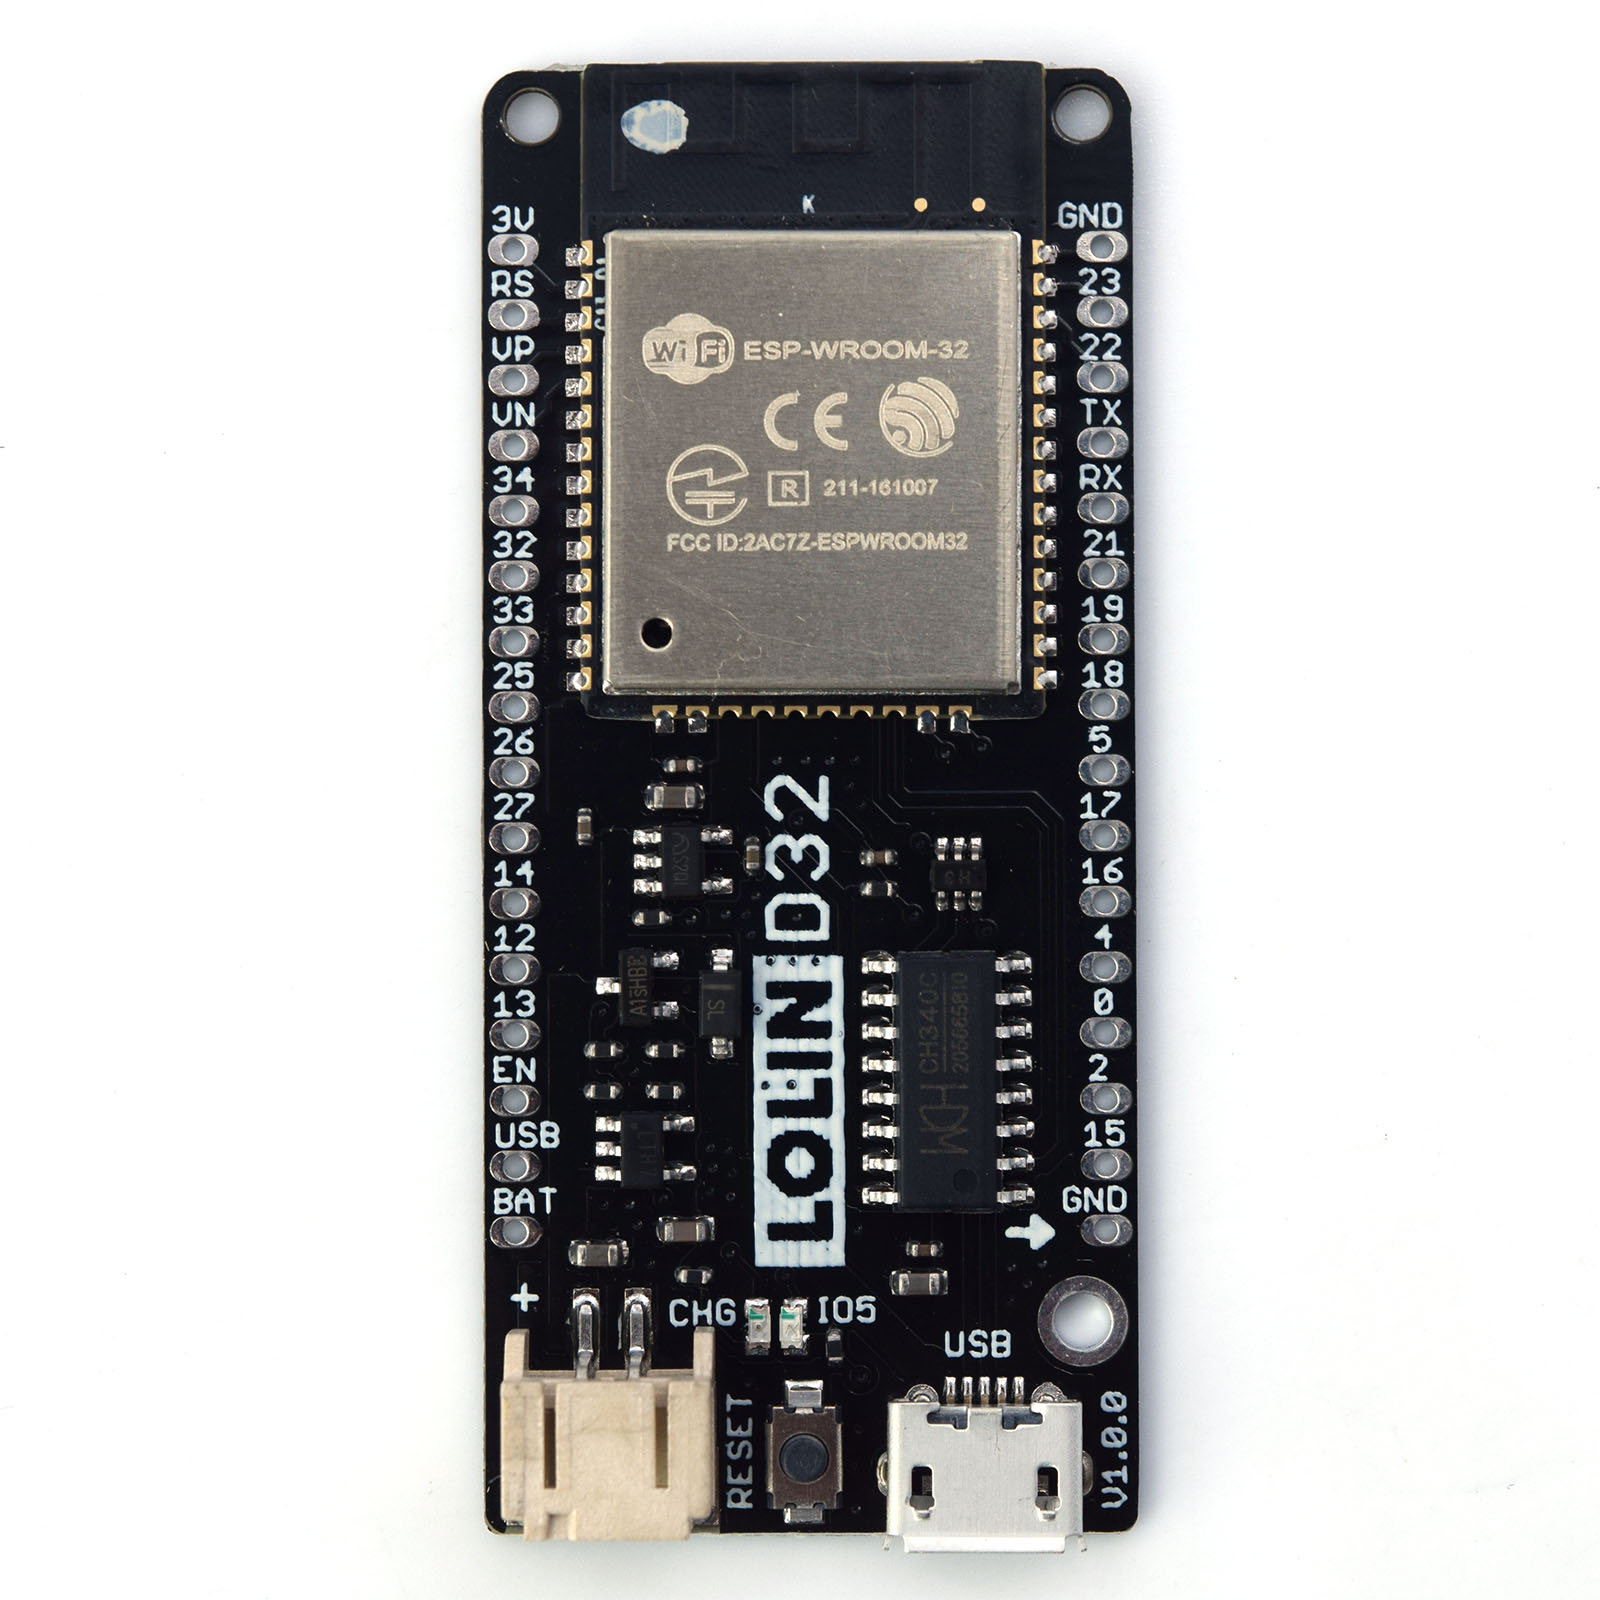
\includegraphics[scale=0.5]{images/d32_lolin}
    \caption{ESP32 pločica (Izvor:~\cite{wemos-docs})}
\end{figure}

Uz glavnu pločicu potreban je i takozvani \textit{power shield} koji omogućava napajanje od 12V\@.
Komponenta nije uključena u standardni paket WEMOS D32, a potrebna je zbog električne brave koja radi na 12V\@.

\subsection{MFRC522}

Kreditne kartice sadrže RFID čip u kojem je pohranjen jedinstveni identifikator kartice (UID).
Za autorizaciju pristupa sefu potrebno je pročitati UID s čitačem RFID kartica.

\begin{figure}[h!]
    \centering
    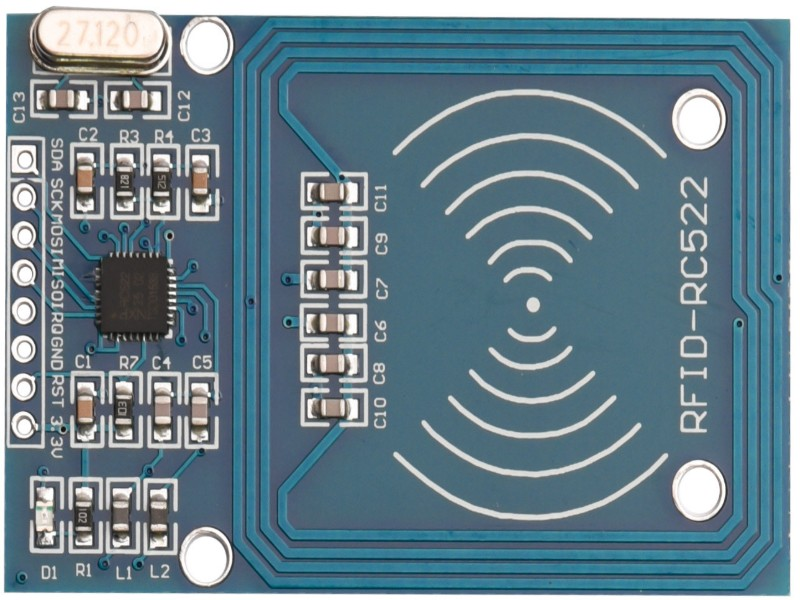
\includegraphics[scale=0.25]{images/mfrc522}
    \caption{MFRC522 čitač (Izvor:~\cite{mfrc522-eradionica})}
\end{figure}

\subsection{Mikroprekidač}

Magnetski mikroprekidač je dvodijelna komponenta koja zatvara strujni krug kad su obje komponente blizu jedna drugoj
(oko 20 milimetara).
Jednostavna komponenta koja služi za određivanje stanja sefa (otvoren ili zatvoren).
Proizvođač je tvrtka \textit{SparkFun}.

\begin{figure}[h!]
    \centering
    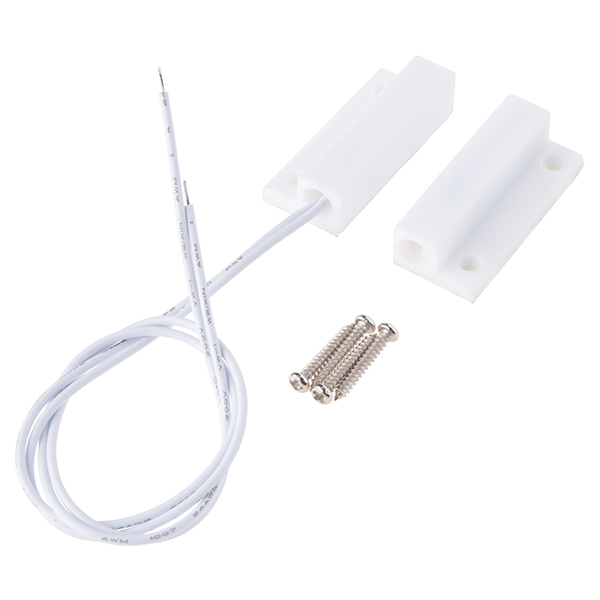
\includegraphics{images/magnetic-switch}
    \caption{Magnetski mikroprekidač (Izvor:~\cite{sparkfun-switch})}
\end{figure}

\pagebreak

\subsection{RGB LED}

LED dioda koja podržava RGB spektar boja.
Komponenta služi kao informacija korisniku o uspješnosti otvaranja sefa.

\begin{figure}[h!]
    \centering
    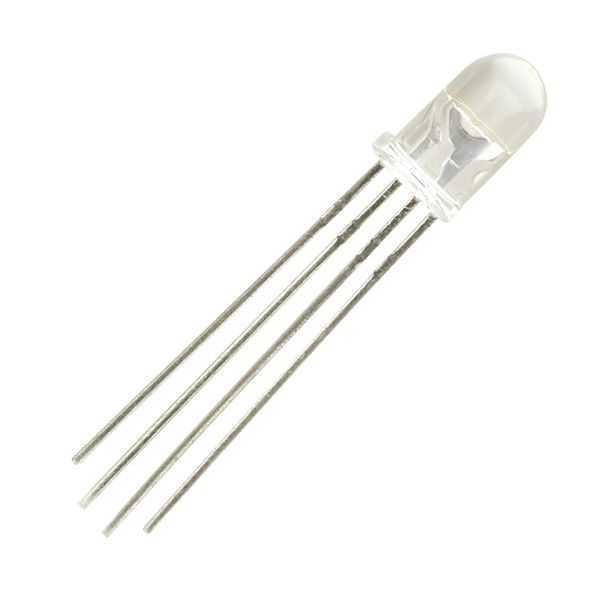
\includegraphics[scale=0.7]{images/rgb-led}
    \caption{RGB LED (Izvor:~\cite{robotistan-led})}
\end{figure}

\subsection{Brava i relej}

Električna brava koja radi na 12V i 500mA\@.
Kad relej zatvori strujni krug brava se otvara i omogućava korisniku pristup sefu.

\begin{figure}[h!]
    \centering
    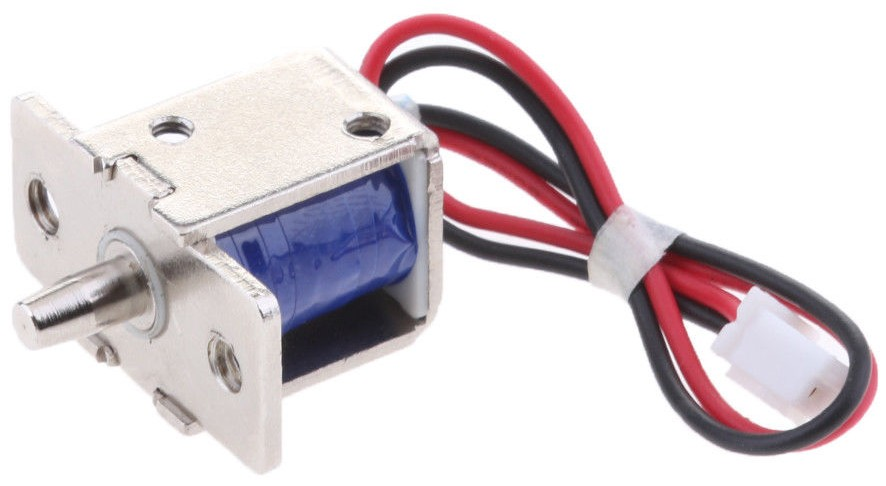
\includegraphics[width=200pt]{images/door-lock}
    \caption{Brava (Izvor:~\cite{ebay-doorlock})}
\end{figure}

\begin{figure}[h!]
    \centering
    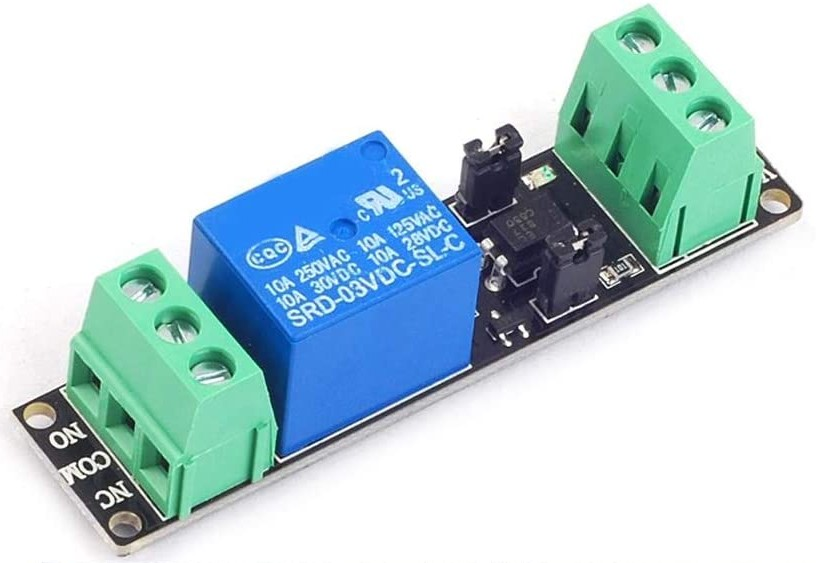
\includegraphics[width=200pt]{images/relay}
    \caption{Relej (Izvor:~\cite{amazon-relay})}
\end{figure}

\pagebreak

\subsection{Napajanje}

Većina komponenti zahtjeva 3.3V napajanje, no električna brava radi na 12V pa zahtjeva vanjsko napajanje.
Potrebno je vanjsko napajanje koje pretvara 220V u 12V\@.

\begin{figure}[h!]
    \centering
    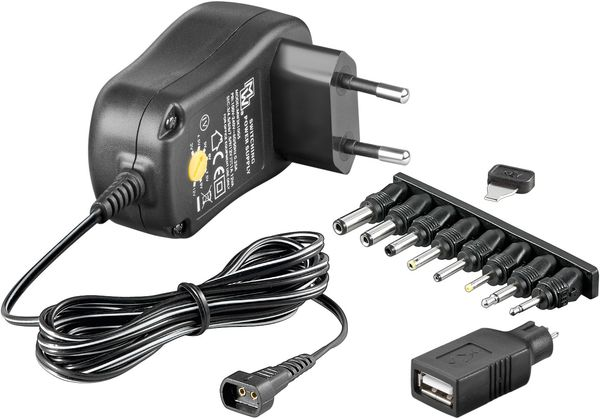
\includegraphics[scale=0.4]{images/power-supply}
    \caption{Napajanje (Izvor:~\cite{chipoteka-power-supply})}
\end{figure}
